\documentclass[12pt,a4paper]{article}

% Packages
\usepackage[utf8]{inputenc}
\usepackage[T1]{fontenc}
\usepackage[english]{babel}
\usepackage{graphicx}
\usepackage{listings}
\usepackage{xcolor}
\usepackage{hyperref}
\usepackage{geometry}
\usepackage{fancyhdr}
\usepackage{titlesec}
\usepackage{float}
\usepackage{caption}
\usepackage{subcaption}
\usepackage{parskip}
\usepackage{microtype}

% Page geometry
\geometry{margin=2.5cm, headheight=15pt}

% Colors for code
\definecolor{codegreen}{rgb}{0,0.6,0}
\definecolor{codegray}{rgb}{0.5,0.5,0.5}
\definecolor{codepurple}{rgb}{0.58,0,0.82}
\definecolor{codeblue}{rgb}{0.13,0.29,0.53}
\definecolor{codeorange}{rgb}{0.8,0.4,0}
\definecolor{backcolour}{rgb}{0.97,0.97,0.97}
\definecolor{framecolor}{rgb}{0.8,0.8,0.8}

% Define JavaScript/TypeScript
\lstdefinelanguage{JavaScript}{
  keywords={break, case, catch, continue, debugger, default, delete, do, else, finally, for, function, if, in, instanceof, new, return, switch, this, throw, try, typeof, var, void, while, with, let, const, class, export, extends, import, super, implements, interface, package, private, protected, public, static, yield, async, await, of, from, as, get, set, type, readonly, enum, abstract, declare, module, namespace, require},
  sensitive=true,
  comment=[l]{//},
  morecomment=[s]{/*}{*/},
  morestring=[b]',
  morestring=[b]",
  morestring=[b]`
}

% Define CSS
\lstdefinelanguage{CSS}{
  keywords={color, background, background-color, margin, padding, font, font-size, font-weight, border, border-radius, width, height, display, position, top, left, right, bottom, flex, grid, transition, transform, opacity, z-index, overflow, text-align, line-height, box-shadow, content, cursor, visibility, list-style, text-decoration, vertical-align, white-space, word-wrap, min-width, max-width, min-height, max-height, justify-content, align-items, flex-direction, flex-wrap, gap, var, hsl, rgb, rgba},
  sensitive=true,
  morecomment=[l]{//},
  morecomment=[s]{/*}{*/},
  morestring=[b]',
  morestring=[b]"
}

% Code listing style
\lstdefinestyle{mystyle}{
    backgroundcolor=\color{backcolour},
    commentstyle=\itshape\color{codegreen},
    keywordstyle=\bfseries\color{codeblue},
    numberstyle=\scriptsize\color{codegray},
    stringstyle=\color{codeorange},
    basicstyle=\ttfamily\small,
    breakatwhitespace=false,
    breaklines=true,
    captionpos=b,
    keepspaces=true,
    numbers=left,
    numbersep=8pt,
    showspaces=false,
    showstringspaces=false,
    showtabs=false,
    tabsize=2,
    frame=single,
    framerule=0.5pt,
    rulecolor=\color{framecolor},
    xleftmargin=15pt,
    framexleftmargin=15pt,
    aboveskip=12pt,
    belowskip=8pt,
    abovecaptionskip=8pt
}
\lstset{style=mystyle}

% Header and footer
\pagestyle{fancy}
\fancyhf{}
\fancyhead[L]{\small\textit{Distributed Systems Lab}}
\fancyhead[R]{\small\textit{Conference Management System}}
\fancyfoot[C]{\thepage}
\renewcommand{\headrulewidth}{0.4pt}
\renewcommand{\footrulewidth}{0.4pt}

% Title formatting
\titleformat{\section}{\Large\bfseries\color{codeblue}}{\thesection}{1em}{}[\vspace{0.5em}\hrule\vspace{0.5em}]
\titleformat{\subsection}{\large\bfseries}{\thesubsection}{1em}{}
\titleformat{\subsubsection}{\normalsize\bfseries}{\thesubsubsection}{1em}{}

% Hyperref setup
\hypersetup{
    colorlinks=true,
    linkcolor=codeblue,
    filecolor=magenta,
    urlcolor=codeblue,
    citecolor=codeblue,
    pdftitle={Conference Management System Report},
    pdfauthor={Student Name}
}

% Fix overfull hboxes
\sloppy

\begin{document}

% ============================================
% TITLE PAGE
% ============================================
\begin{titlepage}
    \centering
    \vspace*{1cm}
    
    {\Large\textsc{Universite Hassan II de Casablanca}}\\[0.3cm]
    {\large\textsc{ENSET Mohammedia}}\\[0.5cm]
    {\large Master's Program in Software Engineering (SDIA)}\\[2cm]
    
    \rule{\textwidth}{1.5pt}\\[0.5cm]
    {\Huge\bfseries Design and Implementation of a\\[0.3cm] Conference Management Microservices System}\\[0.5cm]
    \rule{\textwidth}{1.5pt}\\[1.5cm]
    
    {\Large\textsc{Distributed Systems Laboratory}}\\[3cm]
    
    \begin{minipage}{0.5\textwidth}
        \begin{flushleft}
            \large\textbf{Prepared by:}\\[0.3cm]
            \Large Otmane TOUHAMI
        \end{flushleft}
    \end{minipage}
    \hfill
    \begin{minipage}{0.4\textwidth}
        \begin{flushright}
            \large\textbf{Academic Year:}\\[0.3cm]
            \Large 2024 -- 2025
        \end{flushright}
    \end{minipage}
    
    \vfill
    
    {\large Academic Year 2024 -- 2025}
    
\end{titlepage}

% ============================================
% ABSTRACT
% ============================================
\newpage
\thispagestyle{empty}
\vspace*{3cm}
\begin{center}
    {\Large\bfseries Abstract}
\end{center}
\vspace{1cm}

\noindent
This report details the design and implementation of a scalable, microservices-based Conference Management System. The project aims to provide a comprehensive platform for managing academic conferences, keynote speakers, and participant reviews.

\vspace{0.5cm}
\noindent
The architecture leverages the Spring Cloud ecosystem to solve distributed system challenges such as service discovery, configuration management, and intelligent routing. The backend comprises specialized microservices: a \textbf{Conference Service} for event management and reviews, and a \textbf{Keynote Service} for speaker profiles. These services communicate securely using OpenFeign and are protected by OAuth2/OIDC authentication via Keycloak.

\vspace{0.5cm}
\noindent
A modern frontend application, built with Angular 19 and a reactive signals-based architecture, provides an intuitive user interface. The system ensures high availability and resilience through patterns like Circuit Breakers (Resilience4j) and is containerized using Docker for reproducible deployment.

\vspace{2cm}
\noindent\textbf{Keywords:} Microservices, Spring Boot, Spring Cloud, Angular, Keycloak, Docker, Resilience4j, Feign Client.

% ============================================
% TABLE OF CONTENTS
% ============================================
\newpage
\tableofcontents
\newpage

% ============================================
\section{Introduction}
% ============================================

In the domain of academic event management, systems must handle complex data relationships and varying loads while maintaining data consistency and user accessibility. Monolithic architectures often struggle to scale specific components independently or adopt new technologies for isolated features.

This laboratory project addresses these challenges by implementing a decoupled microservices architecture. The system facilitates the creation and management of conferences, the assignment of keynote speakers, and the submission of attendee reviews.

The primary objectives are:
\begin{enumerate}
    \item To implement a robust microservices infrastructure using Spring Cloud (Gateway, Eureka, Config).
    \item To secure the application using industry-standard OAuth2/OIDC protocols with Keycloak.
    \item To demonstrate effective inter-service communication and fault tolerance.
    \item To develop a responsive, user-friendly frontend using Angular.
\end{enumerate}

% ============================================
\section{System Architecture}
% ============================================

The system is designed as a set of loosely coupled services that collaborate to fulfill business requirements.

\subsection{Architecture Overview}

The architecture diagram below illustrates the interactions between the client (Angular), the infrastructure services, and the core business microservices.

\begin{figure}[H]
    \centering
    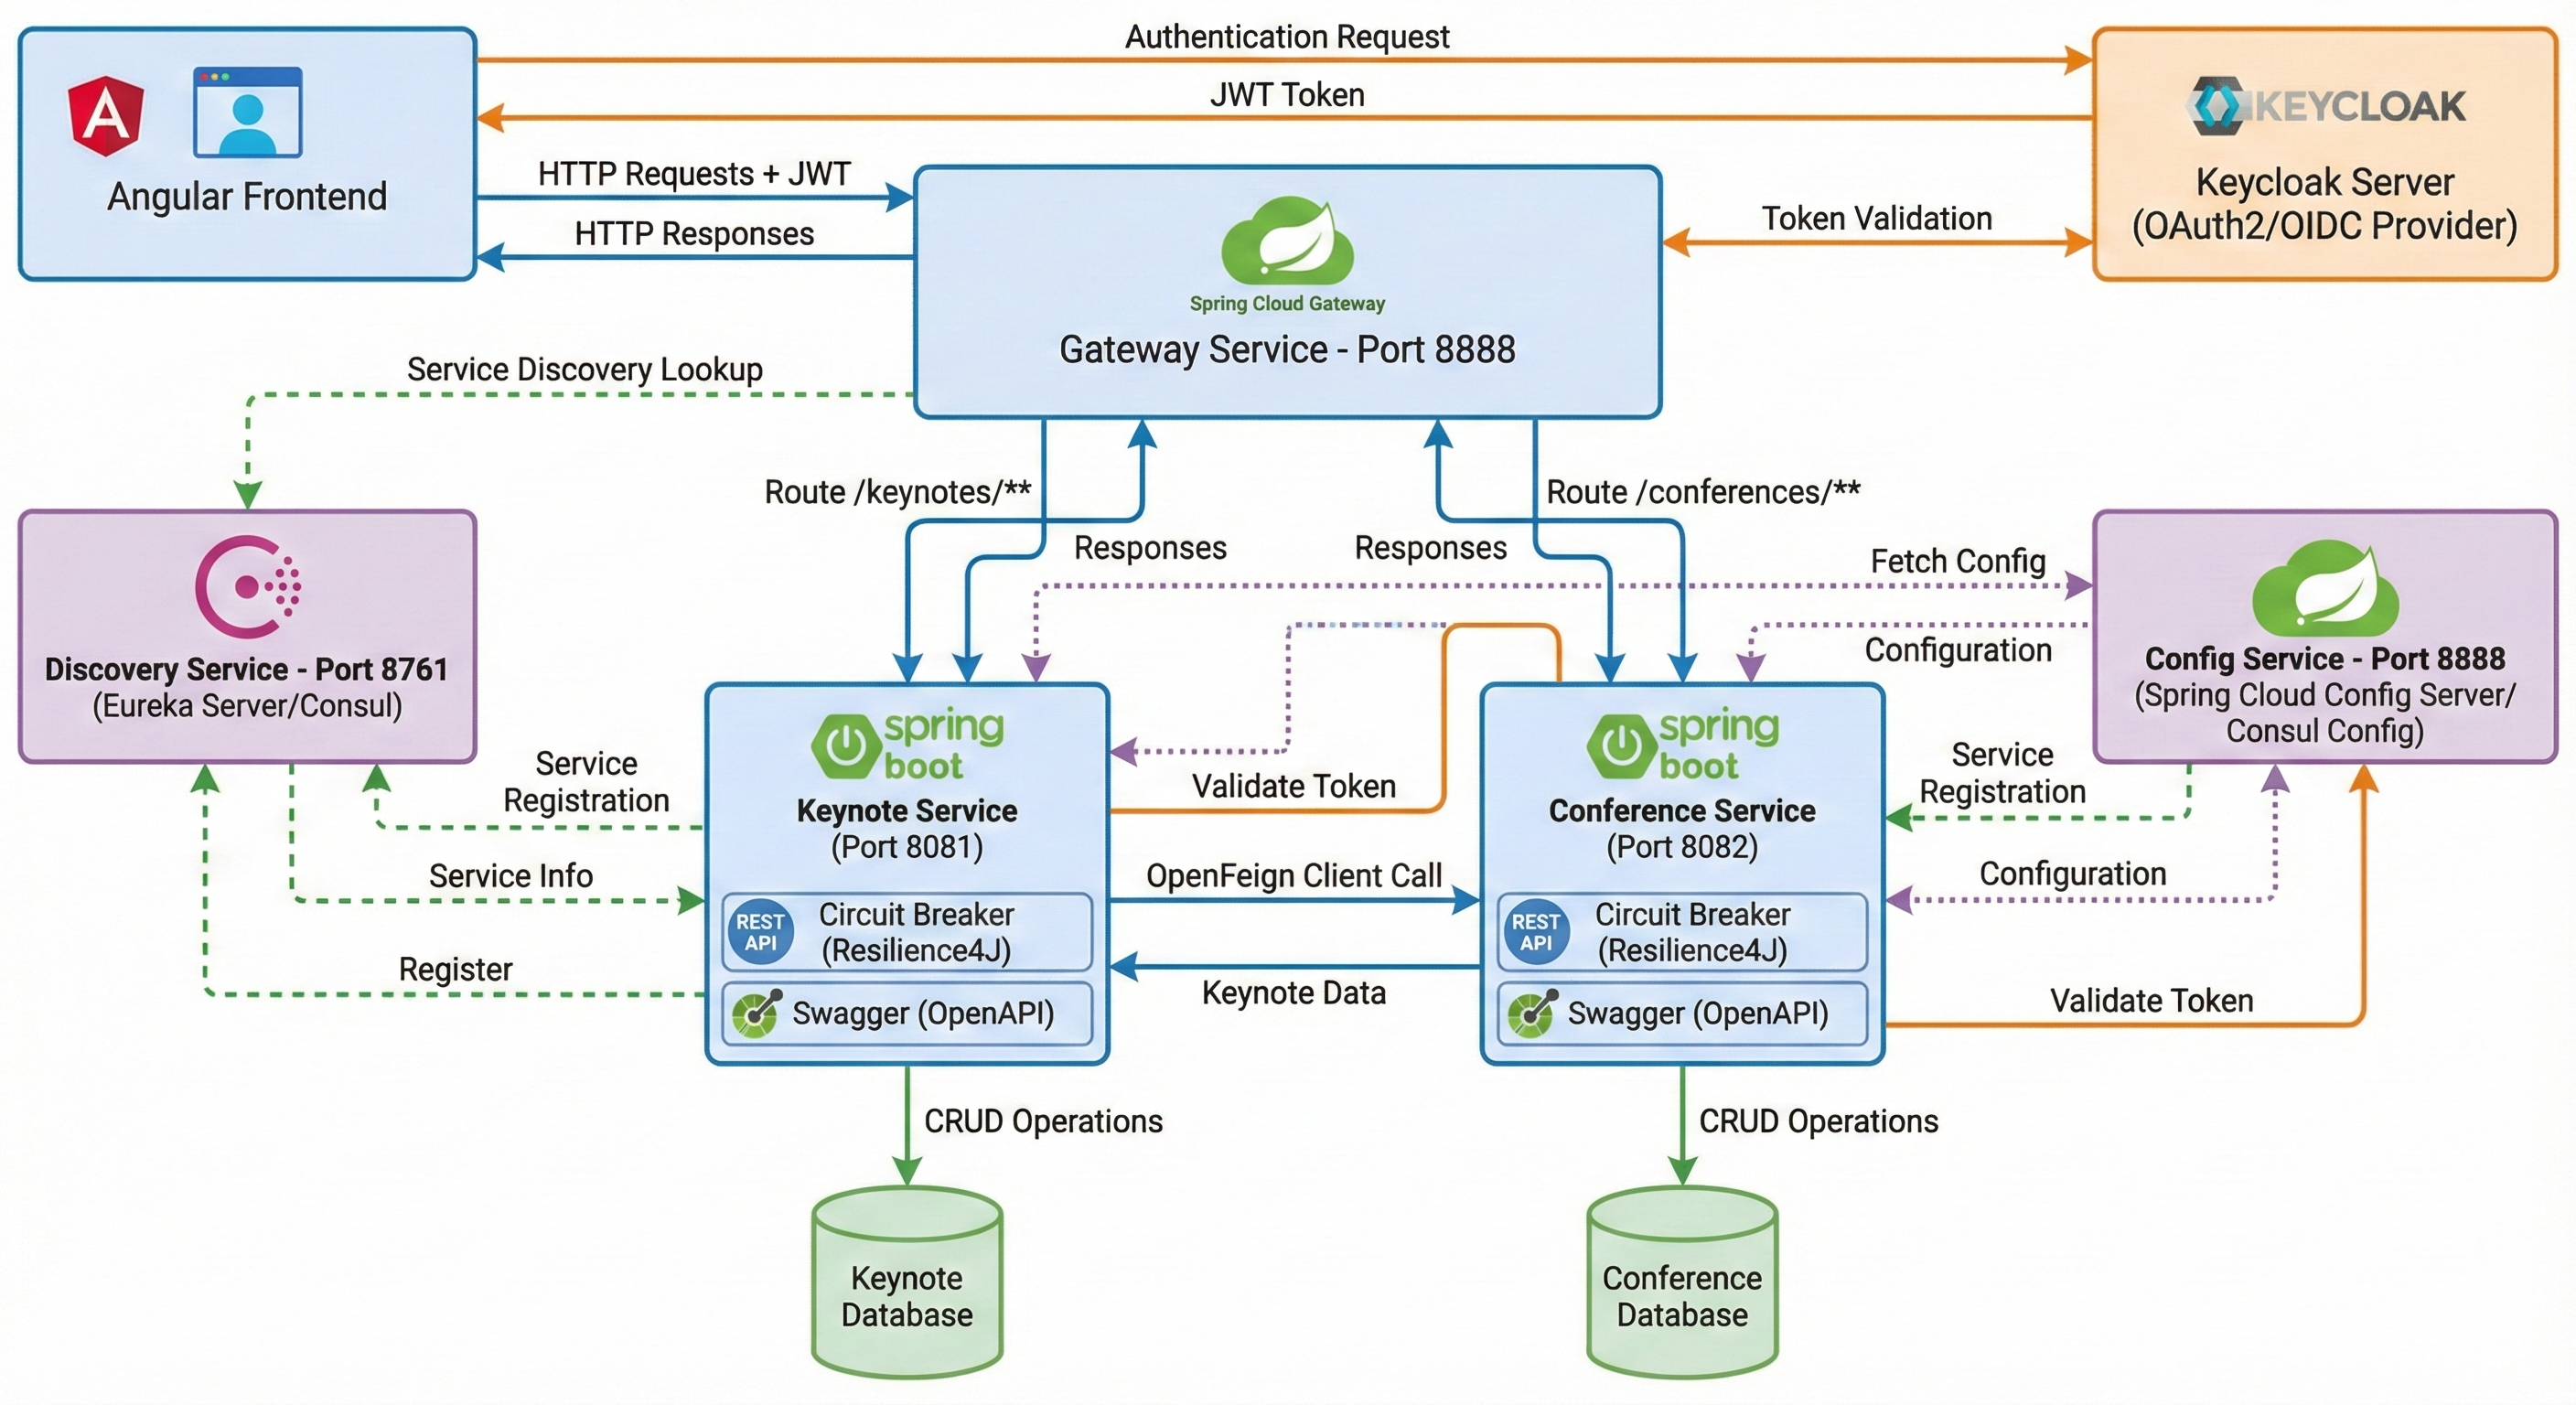
\includegraphics[width=\textwidth]{../screenshots/architecture.png}
    \caption{Global Architecture of the Conference Management System}
    \label{fig:architecture}
\end{figure}

Data flows from the client through the \textbf{API Gateway}, which handles routing and initial security checks. The gateway discovers service locations via the \textbf{Discovery Service} (Eureka). All services retrieve their configuration from the \textbf{Config Service}. The \textbf{Keycloak} server acts as the Identity Provider (IdP), issuing JWT tokens for authentication.

\subsection{Technology Stack}
\begin{itemize}
    \item \textbf{Backend Language}: Java 21
    \item \textbf{Framework}: Spring Boot 3.4.1, Spring Cloud 2024.0.0
    \item \textbf{Database}: H2 (In-memory for development/testing)
    \item \textbf{Security}: Spring Security 6, OAuth2 Resource Server, Keycloak
    \item \textbf{Frontend}: Angular 19 (TypeScript, Signals)
    \item \textbf{Containerization}: Docker, Docker Compose
\end{itemize}

% ============================================
\section{Infrastructure Services}
% ============================================

The infrastructure layer provides the operational foundation for the microservices.

\subsection{Service Discovery (Netflix Eureka)}
The Discovery Service allows microservices to register themselves and discover other services dynamically. This eliminates the need for hardcoded hostnames and ports.

\subsection{Configuration Management (Spring Cloud Config)}
The Config Service centralizes application configuration. It serves properties from a git repository (or local filesystem), allowing configuration updates without recompiling services.

\subsection{API Gateway (Spring Cloud Gateway)}
The Gateway Service acts as the single entry point. It routes requests to the appropriate microservice based on the URL path (e.g., \texttt{/api/v1/conferences} $\rightarrow$ \texttt{conference-service}) and handles Cross-Origin Resource Sharing (CORS).

\subsection{Security \& Identity (Keycloak)}
Keycloak manages users, roles (ADMIN, USER), and authentication. The backend services act as Resource Servers, validating the JWT tokens attached to incoming requests.

\begin{figure}[H]
    \centering
    \includegraphics[width=0.8\textwidth]{../screenshots/keycloak-login-ui.png}
    \caption{Keycloak Login Interface}
    \label{fig:keycloak}
\end{figure}

% ============================================
\section{Business Services Implementation}
% ============================================

The core logic is divided into two main services.

\subsection{Conference Service}
This service manages conference details and reviews. It owns the \texttt{Conference} and \texttt{Review} entities.

\subsubsection{Entity Model}
The \texttt{Conference} entity includes a reference to a Keynote speaker (\texttt{keynoteId}) stored as a UUID, adhering to the database-per-service pattern where foreign keys to other services' tables are avoided.

\begin{lstlisting}[language=Java, caption=Conference Entity]
@Entity
@Getter @Setter @AllArgsConstructor @NoArgsConstructor @Builder
public class Conference {
    @Id
    @GeneratedValue(strategy = GenerationType.UUID)
    private UUID id;

    @Column(nullable = false)
    private String title;

    @Enumerated(EnumType.STRING)
    private ConferenceType type;

    @OneToMany(mappedBy = "conference", cascade = CascadeType.ALL)
    private List<Review> reviews = new ArrayList<>();

    @Column(name = "keynote_id")
    private UUID keynoteId; // Reference to remote Keynote entity
}
\end{lstlisting}

\subsection{Keynote Service}
This service manages the profiles of keynote speakers (name, email, function). It exposes a REST API for CRUD operations on speakers.

\subsection{Inter-Service Communication}
The Conference Service needs to display speaker details. It uses \textbf{Spring Cloud OpenFeign} to call the Keynote Service. To handle network failures, **Resilience4j** is used as a circuit breaker.

\begin{lstlisting}[language=Java, caption=Keynote Feign Client with Circuit Breaker]
@FeignClient(name = "keynote-service")
public interface KeynoteClient {
    Logger log = LoggerFactory.getLogger(KeynoteClient.class);

    @GetMapping("/api/v1/keynotes/{id}")
    @CircuitBreaker(name = "keynoteService", fallbackMethod = "getKeynoteByIdFallback")
    KeynoteResponseDto getKeynoteById(@PathVariable UUID id);

    default KeynoteResponseDto getKeynoteByIdFallback(UUID id, Exception e) {
        log.error("Fallback triggered for id " + id, e);
        return KeynoteResponseDto.builder()
                .firstName("Unknown")
                .lastName("Speaker")
                .build();
    }
}
\end{lstlisting}

\subsubsection{Security Context Propagation}
Since Feign clients run in a protected environment, the JWT token must be forwarded to the downstream service. We implemented a \texttt{RequestInterceptor} to propagate the \texttt{Authorization} header. Additionally, \texttt{SecurityContextHolder} strategy was set to \texttt{MODE\_INHERITABLETHREADLOCAL} to ensure the context is available in Resilience4j's thread pool.

% ============================================
\section{Frontend Application}
% ============================================

The Angular frontend provides a seamless user experience, interacting with the backend services via the API Gateway.

\subsection{User Interface Design}
The application features a modern, responsive design.

\begin{figure}[H]
    \centering
    \includegraphics[width=0.9\textwidth]{../screenshots/landing-page.png}
    \caption{Application Landing Page}
    \label{fig:landing}
\end{figure}

\begin{figure}[H]
    \centering
    \includegraphics[width=0.9\textwidth]{../screenshots/conferences-page.png}
    \caption{Conference Listing Page}
    \label{fig:conferences}
\end{figure}

\subsection{Detailed Views}
The Conference Detail page aggregates information. It displays the conference metadata, the fetched Keynote Speaker profile, and a grid of participant reviews.

\begin{figure}[H]
    \centering
    \includegraphics[width=0.9\textwidth]{../screenshots/conference-detail-page.png}
    \caption{Conference Details with Keynote and Reviews Grid}
    \label{fig:conf-detail}
\end{figure}

The "Reviews" section demonstrates the 3-column grid layout implemented using CSS Grid, which responsive adapts to mobile and tablet screens.

% ============================================
\section{Deployment}
% ============================================

The entire system is containerized using Docker. A \texttt{docker-compose.yml} file orchestrates the deployment of all microservices, databases, Keycloak, and the frontend (served via Nginx).

\begin{lstlisting}[caption=Docker Compose Extract]
services:
  gateway-service:
    build: ./backend/gateway-service
    ports:
      - "8888:8888"
    depends_on:
      - discovery-service
      - keycloak

  frontend:
    build: ./frontend
    ports:
      - "4200:80"
    depends_on:
      - gateway-service

  conference-service:
    build: ./backend/conference-service
    environment:
      - SPRING_CONFIG_IMPORT=configserver:http://config-service:9999/
\end{lstlisting}

This setup allows for a single-command deployment using \texttt{docker-compose up -d --build}, significantly simplifying the development and testing workflow.

% ============================================
\section{Conclusion}
% ============================================

The Conference Management System successfully demonstrates the principles of microservices architecture. By decomposing the application into focused services, we improved modularity and maintainability. Implementing OpenFeign and Resilience4j ensured robust inter-service communication, while Keycloak provided a secure and standardized authentication mechanism.

The project highlights the complexity of distributed systems—specifically regarding data consistency, security context propagation, and configuration management—and presents effective solutions using the Spring Cloud ecosystem. The modern Angular frontend complements this robust backend, delivering a professional and responsive user experience.

\end{document}
